\documentclass[14pt,aspectratio=1610]{beamer}

\usepackage[brazil]{babel}
\usepackage[utf8]{inputenc}
%\UseRawInputEncoding
\usepackage[T1]{fontenc}
%\usepackage{Sweave}
%\usepackage{animate}
\usepackage{amsbsy}
\usepackage{amsfonts}
\usepackage{amsmath}
\usepackage{amssymb}
\usepackage{amsthm}
\usepackage[toc,page,title,titletoc]{appendix}
%\usepackage[fixlanguage]{babelbib}
%\usepackage[pdftex]{color}
\usepackage{dsfont}
\usepackage{esvect}
\usepackage[labelfont=bf]{caption}
\usepackage{subcaption}
\usepackage{float}
\usepackage[Glenn]{fncychap}%Sonny %Conny %Lenny %Glenn %Renje %Bjarne %Bjornstrup
%\usepackage{geometry, calc, color, setspace}%
%\geometry{a4paper, headsep=1.0cm, footskip=1cm, lmargin=3cm, rmargin=2cm, tmargin=3cm, bmargin=2cm}
\usepackage{graphicx}
\usepackage{indentfirst}%Para indentar os parágrafos automáticamente
\usepackage{lipsum}
\usepackage{longtable}
\usepackage{mathtools}
\usepackage{listings}%Inserir codigo do R no latex
%\usepackage{slashbox}
\usepackage{multirow}
\usepackage{multicol}
\usepackage{natbib}
\setcitestyle{authoryear,open={(},close={)}} %Citation-related commands
\bibliographystyle{abbrvnat}
%\usepackage{csquotes}
%\usepackage[natbib=true,style=abnt, sorting=none]{biblatex}
%\addbibresource{bibliografia.bib}
\usepackage[figuresright]{rotating}
\usepackage{spalign}
%\usepackage{pgfpages}
\usepackage{pgfplots}
\pgfplotsset{compat=1.18}
\usepackage{tikz}
\usepackage{color, colortbl}
\usepackage{ragged2e}%para justificar o texto dentro de algum ambiente
\definecolor{Gray}{gray}{0.9}
\definecolor{LightCyan}{rgb}{0.88,1,1}
\definecolor{Lightblue}{RGB}{50, 149, 168}
%\usepackage{grffile}

\usepackage[all]{xy}



\usetheme{Madrid}
\usecolortheme[RGB={193,0,0}]{structure}

%\setbeamertemplate{footline}[frame number]
%\setbeamertemplate{footline}[text line]{%
%  \parbox{\linewidth}{\vspace*{-8pt}\hfill\date{}\hfill\insertshortauthor\hfill\insertpagenumber}}
\beamertemplatenavigationsymbolsempty
\renewcommand{\vec}[1]{\mbox{\boldmath$#1$}}
\newtheorem{Teorema}{Teorema}
\newtheorem{Proposicao}{Proposição}
\newtheorem{Definicao}{Definição}
\newtheorem{Corolario}{Corolário}
\newtheorem{Demonstracao}{Demonstração}
\newcommand{\bx}{\ensuremath{\bar{x}}}
\newcommand{\Ho}{\ensuremath{H_{0}}}
\newcommand{\Hi}{\ensuremath{H_{1}}}
\everymath{\displaystyle}

\apptocmd{\frame}{}{\justifying}{} % Allow optional arguments after frame.

\title{Estatística I}
\author{Prof. Fernando de Souza Bastos \texorpdfstring{\\ fernando.bastos@ufv.br}{}}
\institute{Departamento de Estatística \texorpdfstring{\\ Universidade Federal de Viçosa}{}\texorpdfstring{\\ Campus UFV - Viçosa}{}}
\date{}
\newcommand\mytext{Aula 20}
\newcommand\mytextt{Fernando de Souza Bastos}
\newcommand\mytexttt{\url{https://ufvest.github.io/}}

\makeatletter
\setbeamertemplate{footline}
{
  \leavevmode%
  \hbox{%
  \begin{beamercolorbox}[wd=.3\paperwidth,ht=2.25ex,dp=1ex,center]{author in head/foot}%
    \usebeamerfont{author in head/foot}\mytext
  \end{beamercolorbox}%
  \begin{beamercolorbox}[wd=.3\paperwidth,ht=2.25ex,dp=1ex,center]{title in head/foot}%
    \usebeamerfont{title in head/foot}\mytextt
  \end{beamercolorbox}%
  \begin{beamercolorbox}[wd=.35\paperwidth,ht=2.25ex,dp=1ex,right]{site in head/foot}%
    \usebeamerfont{site in head/foot}\mytexttt\hspace*{2em}
    \insertframenumber{} / \inserttotalframenumber\hspace*{2ex} 
  \end{beamercolorbox}}%
  \vskip0pt%
}
\makeatother

\providecommand{\arcsin}{} \renewcommand{\arcsin}{\hspace{2pt}\textrm{arcsen}}
\providecommand{\sin}{} \renewcommand{\sin}{\hspace{2pt}\textrm{sen}}
%\newtheorem{Teorema}{Teorema}
%\newtheorem{Proposicao}{Proposição}
%\newtheorem{Definicao}{Definição}
%\newtheorem{Corolario}{Corolário}
%\newtheorem{Demonstracao}{Demonstração}

\titlegraphic{\hspace*{8cm}\href{https://fsbmat-ufv.github.io/}{
\includegraphics[width=2cm]{Figuras/mylogo.png}}
}


\usepackage{hyperref,bookmark}
\hypersetup{
  colorlinks=true,
  linkcolor=blue,
  citecolor=red,
  filecolor=blue,
  urlcolor=blue,
}

% Layout da pagina
\hypersetup{pdfpagelayout=SinglePage}
\begin{document}
%\Sconcordance{concordance:Aula21.tex:Aula21.Rnw:%
1 251 1 1 8 1 2 6 0 1 1 9 0 1 3 7 1 1 8 7 0 2 1 5 0 2 1 9 0 1 3 76 1 1 %
2 1 0 5 1 5 0 2 1 5 0 1 1 6 0 1 2 7 1 1 2 1 0 4 1 8 0 1 2 4 0 1 2 6 1 1 %
2 1 0 1 1 9 0 1 2 17 1 1 5 4 0 1 1 8 0 1 2 7 1 1 2 1 0 1 1 8 0 1 1 7 0 %
1 1 7 0 2 1 5 0 2 1 9 0 1 2 9 1}


\frame{\titlepage}

\begin{frame}{}
\frametitle{\bf Sumário}
\tableofcontents
\end{frame}
\section{Regressão Linear Simples}
\begin{frame}{}
\frametitle{ }
\begin{block}{}
\justifying
Em certas situações podemos estar interessados em descrever a relação entre duas variáveis, e também predizer o valor de uma a partir de outra. Por exemplo, se sabemos a altura de um certo estudante, mas não o seu peso, qual seria um bom chute para o peso deste estudante? 
\end{block}
\end{frame}

\begin{frame}[fragile]{}
\frametitle{ }
\begin{block}{}
\begin{center}
%\begin{Schunk}
%\begin{Sinput}

\begin{verbatim}
x = c(176, 154, 138, 196, 132, 176, 181, 169, 150, 175)
y = c(82, 49, 53, 112, 47, 69, 77, 71, 62, 78)
plot(x,y,xlab="Altura (cm)",ylab="Peso (kg)",
      pch=16, ylim = c(40,115))
lines(x, fitted(lm(y ~ x)), col="blue")    
\end{verbatim}

%\end{Sinput}
%\end{Schunk}
\end{center}
\end{block}
\vspace{-1.3cm}
\begin{center}
\setkeys{Gin}{width=0.5\linewidth}
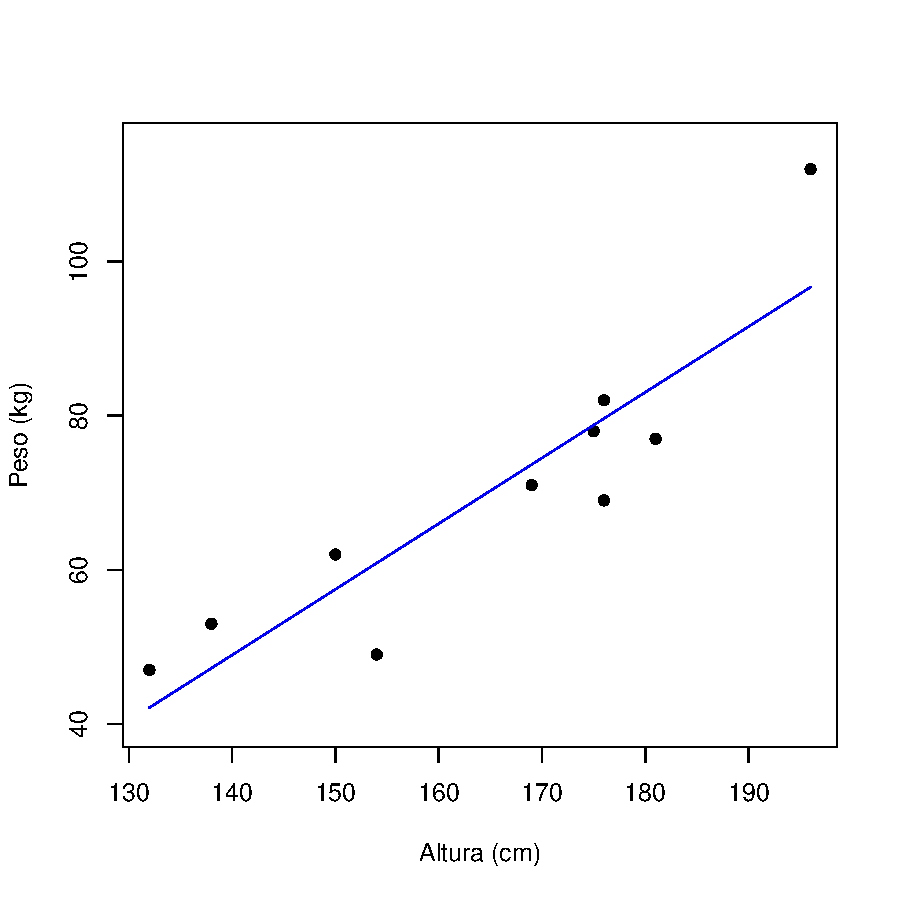
\includegraphics{Figuras/Aula20-002.pdf}
\end{center}
\end{frame}

\begin{frame}[fragile]{}
\frametitle{ }
\begin{block}{}
\begin{center}
%\begin{Schunk}
%\begin{Sinput}
\begin{verbatim}
doses <- c(0, 50, 100, 150, 200, 250, 300)
resp <- c(148.6, 153.6, 154.5, 154.9, 158, 160, 154.4)
reglin <- lm(resp ~ doses) 
plot(doses, resp) #(variável indep. primeiro)
lines(doses, fitted(reglin), col="blue")#acrescenta 
a reta de regressão ajustada
\end{verbatim}
%\end{Sinput}
%\end{Schunk}
\end{center}
\end{block}
\vspace{-1.3cm}
\begin{center}
\setkeys{Gin}{width=0.5\linewidth}
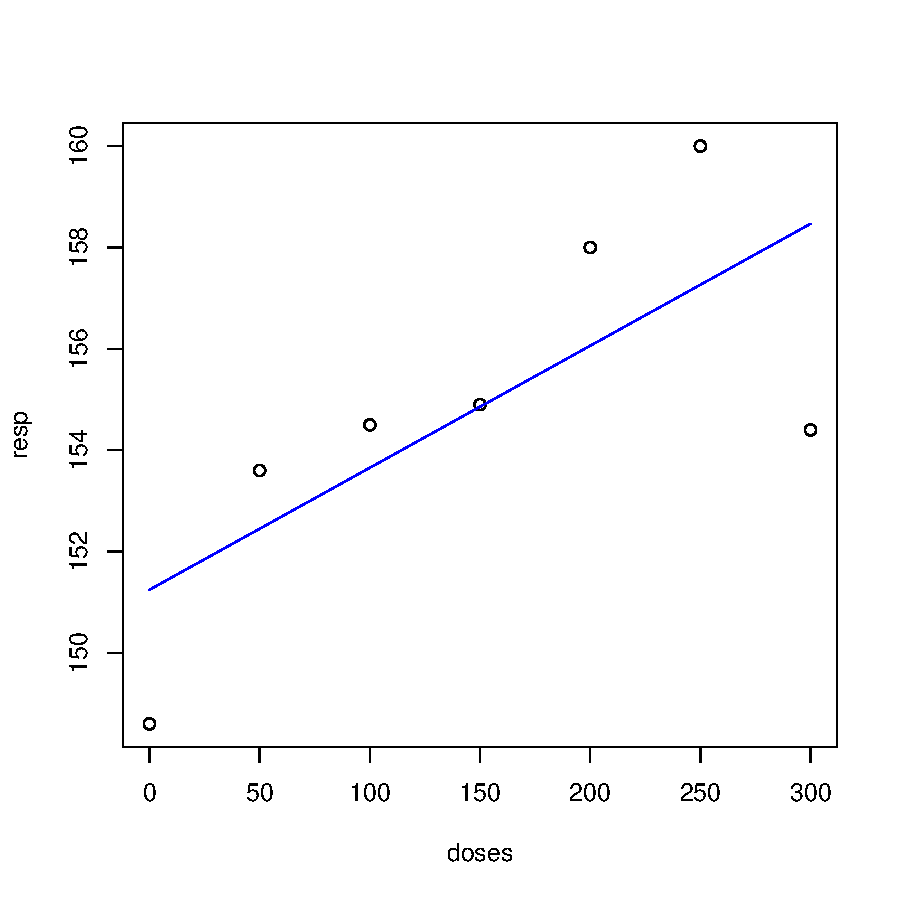
\includegraphics{Figuras/Aula20-004}
\end{center}
\end{frame}

\begin{frame}[fragile]{}
\frametitle{ }
\begin{block}{}
\begin{center}
%\begin{Schunk}
%\begin{Sinput}
\begin{verbatim}
#Tempo de espera entre erupções e a duração da erupção
fit <- lm(waiting~eruptions, data=faithful)
plot(faithful)
lines(faithful$eruptions, fitted(fit), col="blue")
\end{verbatim}
%\end{Sinput}
%\end{Schunk}
\end{center}
\end{block}
\vspace{-1.3cm}
\begin{center}
\setkeys{Gin}{width=0.5\linewidth}
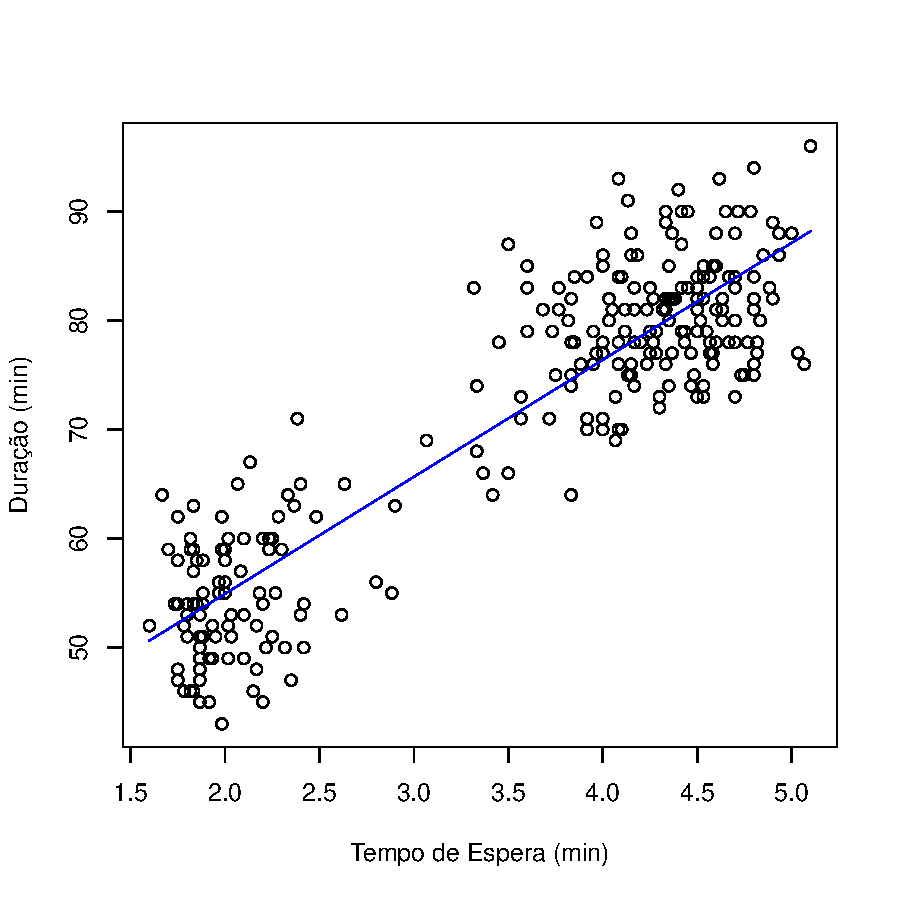
\includegraphics{Figuras/Aula20-006}
\end{center}
\end{frame}

\begin{frame}{}
\frametitle{Objetivos:}
\begin{block}{}
\justifying
Estudar a relação linear entre duas variáveis quantitativas. Exemplos:
\begin{enumerate}[(i)]
\item Altura dos pais e altura dos filhos;\pause
\item Renda semanal e despensas de consumo;\pause
\item Variação dos salários e taxa de desemprego;\pause
\item Demanda dos produtos de uma firma e publicidade;\pause
\end{enumerate}
\end{block}
\begin{block}{}
\justifying
Sob dois pontos de vista:
\begin{enumerate}[(i)]
\item Explicitando a forma dessa relação: regressão.\pause
\item Quantificando a força dessa relação: correlação.
\end{enumerate}
\end{block}
\end{frame}

\begin{frame}{}
\frametitle{ }
\begin{block}{Importante:}
\justifying
Uma relação estatística por sí propria não implica uma causa, para atribuir causa, devemos invocar alguma teoría!
\end{block}
\pause
\begin{block}{}
\justifying
Uma regressão espúria é uma relação estatística existente entre duas variáveis, mas onde não existe nenhuma relação causa-efeito entre elas. Essa relação estatística pode ocorrer por pura coincidência ou por causa de uma terceira variável. Ou seja, neste último caso, pode ocorrer que as variáveis X e Y sejam correlacionadas porque ambas são causadas por uma terceira variável Z.
\end{block}
\end{frame}

\begin{frame}{}
\frametitle{ }
\begin{block}{}
\justifying
Só porque (A) acontece juntamente com (B) não significa que (A) causa (B). Determinar se existe de fato uma relação de causalidade requer  investigação adicional pois podem acontecer cinco situações:
\begin{enumerate}[(i)]
\item (A) causa realmente (B);\pause
\item (B) pode ser a causa de (A);\pause
\item Um terceiro factor (C) pode ser causa tanto de (A) como de (B);\pause
Pode ser uma combinação das três situações anteriores. Por exemplo, (A) causa (B) e ao mesmo tempo (B) causa também (A);\pause
\item A correlação pode ser apenas uma coincidência, ou seja, os dois eventos não têm qualquer relação para além do fato de ocorrerem ao mesmo tempo. 
\end{enumerate}
\end{block}
\end{frame}

\begin{frame}{}
\frametitle{Exemplos:}
\begin{block}{}
\justifying
``Quanto maiores são os pés de uma criança, maior a capacidade para resolver problemas de matemática. Portanto, ter pés grandes faz ter melhores notas em matemática". 
\end{block}
\end{frame}

\begin{frame}{}
\frametitle{Exemplos:}
\begin{block}{}
\justifying
``Vários estudos apontavam inicialmente que as mulheres em menopausa que recebiam terapia de substituição hormonal (TSH) tinham também um menor risco de doença coronária, o que levou à ideia de que a TSH conferia protecção contra a doença coronária. No entanto, estudos controlados e randomizados (mais rigorosos), feitos posteriormente, mostraram que a TSH causava na verdade um pequeno mas significativo aumento do risco de doença coronária. Uma reanálise dos estudos revelou que as mulheres que recebiam a TSH tinham também uma maior probabilidade de pertencer a uma classe socioeconómica superior, com melhor dieta e hábitos de exercício. A utilização da TSH e a baixa incidência de doença coronária não eram causa e efeito, mas o fruto de uma causa comum". 
\end{block}
\end{frame}

\begin{frame}{}
\frametitle{ }
\begin{block}{}
\justifying
``Quanto menos as pessoas se divorciam em Maine (EUA), menor fica o consumo de margarina naquele Estado". 
\end{block}
\begin{figure}[H]
    \centering
    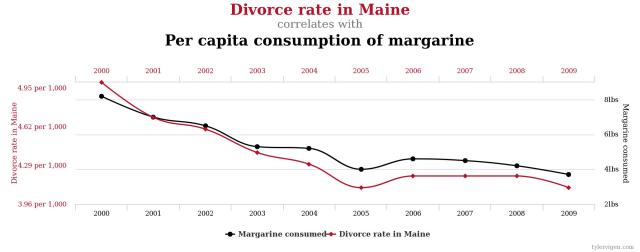
\includegraphics[scale=0.5]{Figuras/Margarina}
    %\caption{Legenda}
    %\label{figRotulo}
\end{figure}
\end{frame}

\begin{frame}{}
\frametitle{ }
\begin{block}{}
\justifying
Deveríamos banir Nicolas Cage do cinema para evitar o afogamento de pessoas? O primeiro gráfico nos dá o número de pessoas afogadas (linha vermelha) e as aparições do Nicolas Cage em filmes (linha preta).
\end{block} 
\begin{figure}[H]
    \centering
    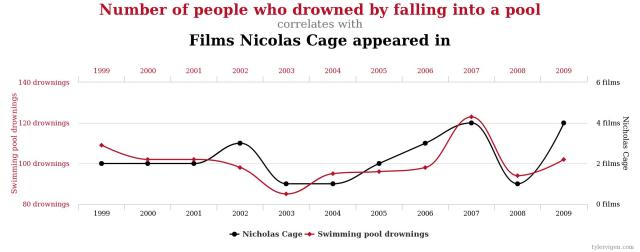
\includegraphics[scale=0.5]{Figuras/Nicolas}
    %\caption{Legenda}
    %\label{figRotulo}
\end{figure}
\end{frame}

\begin{frame}{}
\frametitle{ }
\begin{block}{}
\justifying
Consumo de muçarela (linha vermelha) e doutorados obtidos em engenharia civil (linha preta)
%http://www.tylervigen.com/spurious-correlations
\end{block}
\begin{figure}[H]
    \centering
    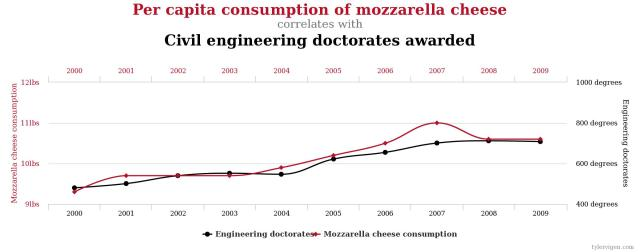
\includegraphics[scale=0.5]{Figuras/Mucarela}
    %\caption{Legenda}
    %\label{figRotulo}
\end{figure}
\end{frame}

\section{Coeficiente de Correlação}
\begin{frame}{Coeficiente de Correlação Amostral de Pearson}
    \begin{block}{}
    \justifying
    O coeficiente de correlação $(r\ \textrm{ou}\ \hat{\rho})$ mede o grau de associação linear entre duas variáveis aleatórias $X$ e $Y.$ Considere,
    \begin{table}[H]
        \centering
        \begin{tabular}{c|cccc}
             $X_{i}$&$X_{1}$ $X_{2}$ $\cdots$ $X_{n}$ \\
             \hline
             $Y_{i}$&$Y_{1}$ $Y_{2}$ $\cdots$ $Y_{n}$ 
        \end{tabular}
    \end{table}
    Assim, o coeficiente de correlação entre $X$ e $Y$ é dado por:
    
    $$r_{XY}=\dfrac{S_{XY}}{\sqrt{S^{2}_{X}\cdot S_{Y}^{2}}}=
    \dfrac{\dfrac{SPD_{XY}}{n-1}}{\sqrt{\dfrac{SQD_{X}}{n-1}\cdot\dfrac{SQD_{Y}}{n-1}}}= 
    \dfrac{SPD_{XY}}{\sqrt{SQD_{X}\cdot SQD_{Y}}}$$
    
    \end{block}
\end{frame}

\begin{frame}{}
\frametitle{}
%\vspace{-0.6cm}
\begin{block}{}
\justifying
Temos,
$$SPD_{XY}=\sum_{i=1}^{n}X_{i}Y_{i}-\dfrac{\Big({\displaystyle\sum_{i=1}^{n}X_{i}}\Big)\Big({\displaystyle\sum_{i=1}^{n}Y_{i}\Big)}}{n}$$
\pause
$$SQD_{X}=\displaystyle{\sum_{i=1}^{n}X_{i}^{2}}-\dfrac{\Big(\displaystyle{\sum_{i=1}^{n}X_{i}}\Big)^{2}}{n}\quad \textrm{e}\quad SQD_{Y}=\displaystyle{\sum_{i=1}^{n}Y_{i}^{2}}-\dfrac{\Big(\displaystyle{\sum_{i=1}^{n}Y_{i}}\Big)^{2}}{n}$$
\end{block}
\pause
\vspace{-0.06cm}
\begin{block}{}
\justifying
$$-1\leq r_{XY}\leq 1$$
\end{block}
%\vspace{-0.8cm}
\end{frame}

\begin{frame}{Exemplo}
\frametitle{}
%\vspace{-0.6cm}
\begin{block}{}
\justifying
\begin{table}[H]
        \centering
        \begin{tabular}{c|cccccc}
             Amostra A&4&8&3&9&7&5 \\
             \hline
             Amostra B&1&5&2&14&3&11 
        \end{tabular}
    \end{table}
\end{block}
\begin{block}{}
\justifying
Temos,
$$SPD_{AB}=\sum_{i=1}^{n}A_{i}B_{i}-\dfrac{\Big({\displaystyle\sum_{i=1}^{n}A_{i}}\Big)\Big({\displaystyle\sum_{i=1}^{n}B_{i}\Big)}}{n}$$
\pause
$$SQD_{A}=\displaystyle{\sum_{i=1}^{n}A_{i}^{2}}-\dfrac{\Big(\displaystyle{\sum_{i=1}^{n}A_{i}}\Big)^{2}}{n}\quad \textrm{e}\quad SQD_{B}=\displaystyle{\sum_{i=1}^{n}B_{i}^{2}}-\dfrac{\Big(\displaystyle{\sum_{i=1}^{n}B_{i}}\Big)^{2}}{n}$$
\end{block}
%\vspace{-0.8cm}
\end{frame}

\begin{frame}{Exemplo}
\frametitle{}
%\vspace{-0.6cm}
\begin{block}{}
\justifying
Assim,
$$SPD_{AB}=252-\dfrac{(36)(36)}{6}=36$$
\pause
$$SQD_{A}=244-\dfrac{(36)^{2}}{6}=28\quad \textrm{e}\quad SQD_{B}=356-\dfrac{(36)^{2}}{6}=140$$
\end{block}
\pause
\begin{block}{}
\justifying
$$r_{AB}=\dfrac{SP_{AB}}{\sqrt{SQD_{A}SQD_{B}}}=\dfrac{36}{\sqrt{28\cdot 140}}=0,5750$$
\end{block}
%\vspace{-0.8cm}
\end{frame}

\section{Modelo de Regressão}
\begin{frame}{Modelo Estatístico}
\frametitle{ }
\begin{block}{}
\justifying
De forma geral, um modelo estatístico pode ser escrito da seguinte forma:

$$Y=\textrm{componente determinística}+\textrm{componente aleatória}$$

existem diversas maneiras de específicar essas componentes. Começaremos com uma regressão linear simples.

\end{block}
\end{frame}


\begin{frame}{}
\frametitle{ }
\begin{block}{}
\justifying
Uma regresão linear simples tem como objetivo aproximar uma variável resposta $Y$ através de uma função linear de uma variável de interesse, ou seja,

$$Y=f(X,\beta)+\varepsilon=\beta_{0}+\beta_{1}X+\varepsilon$$

No qual assume-se que:

\begin{enumerate}[(i)]
\item $E(\varepsilon)=0$\pause
\item $V(\varepsilon)=\sigma^{2}$ (Homocedásticidade)\pause
\item $Cov(\varepsilon_{i},\varepsilon_{j})=0$
\end{enumerate}

em outras palavras, os erros tem média zero, variância constante e são não correlacionados.

\end{block}
\end{frame}

\begin{frame}{}
\frametitle{ }
\begin{block}{}
\justifying
A variável preditora $X$ pode vir de diversas fontes:
\begin{itemize}
\item inputs quantitativos (valores reais, medidas)
\item tranformação de variável quantitativas ($\log()$ ,$\sqrt()$,etc)
\item inputs qualitativos (``dummy" e.x. genêro, classes)
\end{itemize}
Dessa forma, um modelos de regressão consiste em 4 passos:
\begin{enumerate}
\item Escolher o componente determinístico do modelo;\pause
\item Especificar a distribuição do erro;\pause
\item Utilizar os dados para estimar os parâmetros do modelo;\pause
\item Avaliar o modelo estatístico;
\end{enumerate}
\end{block}
\end{frame}


\begin{frame}{}
\frametitle{ }
\begin{block}{}
\justifying
Os dados para a análise de regressão e correlação simples são da forma:
$$(x_{1},y_{1}),(x_{2},y_{2}),\cdots, (x_{n},y_{n})$$

Com base nos dados constrói-se o diagrama de dispersão, que deve exibir
uma tendência linear para que se possa usar a regressão linear.
Este diagrama permite decidir empiricamente:
\begin{itemize}
\item Se um relacionamento linear entre as variáveis $X$ e $Y$ deve ser assumido;
\item Se o grau de relacionamento linear entre as variáveis é forte ou fraco,
conforme o modo como se situam os pontos em redor de uma reta imaginária que passa através do enxame de pontos.
\end{itemize}
\end{block}
\end{frame}

\begin{frame}[fragile]{}
\frametitle{ }
\begin{block}{}
\begin{center}
%\begin{Schunk}
%\begin{Sinput}
\begin{verbatim}
#Encontre o modelo de Regressão Linear que melhor se
ajusta aos dados
x = c(176, 154, 138, 196, 132, 176, 181, 169, 150, 175)
y = c(82, 49, 53, 112, 47, 69, 77, 71, 62, 78)    
\end{verbatim}
%\end{Sinput}
%\end{Schunk}
\end{center}
\end{block}
\vspace{-1.3cm}
\begin{center}
\setkeys{Gin}{width=0.5\linewidth}
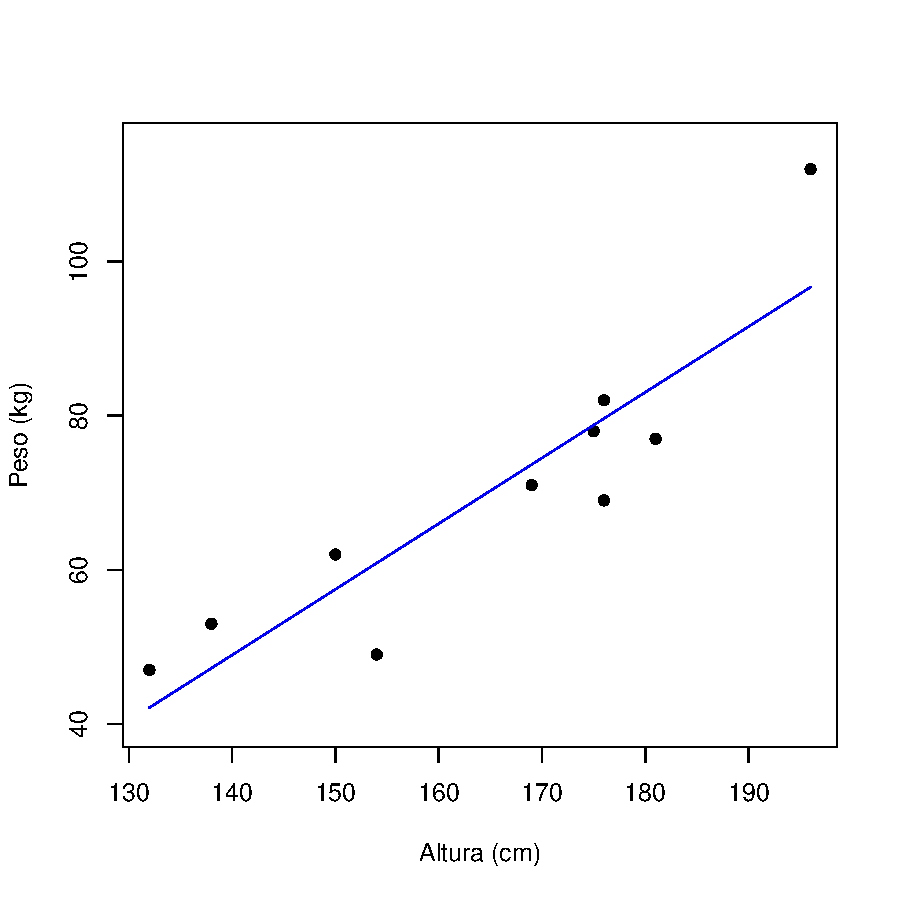
\includegraphics{Figuras/Aula20-008}
\end{center}
\end{frame}

\begin{frame}[fragile]{}
\frametitle{ }
\begin{block}{}
\begin{center}
%\begin{Schunk}
%\begin{Sinput}
\begin{verbatim}
#Encontre o modelo de Regressão Linear que melhor se
ajusta aos dados
x <-  c(176, 154, 138, 196, 132, 176, 181, 169, 150, 175)
y <-  c( 82,  49,  53, 112,  47,  69,  77,  71,  62,  78)
Reg <- lm(y~x)
Reg    
\end{verbatim}
%\end{Sinput}
%\begin{Soutput}
\begin{verbatim}
Call:
lm(formula = y ~ x)

Coefficients:
(Intercept)            x  
   -70.4627       0.8528     
\end{verbatim} 
%\end{Soutput}
%\end{Schunk}
\end{center}
\end{block}
\end{frame}

\begin{frame}[fragile]{}
\frametitle{ }
\begin{block}{}
\begin{center}
%\begin{Schunk}
%\begin{Sinput}
\begin{verbatim}
#library(texreg)
summary(Reg)    
\end{verbatim}
%\end{Sinput}
%\begin{Soutput}
\begin{verbatim}
lm(formula = y ~ x)
Residuals:
     Min       1Q   Median       3Q      Max 
-11.8746  -5.8428   0.7893   4.8001  15.3061 
Coefficients:
            Estimate Std. Error t value Pr(>|t|)    
(Intercept) -70.4627    24.0148  -2.934 0.018878 *  
x             0.8528     0.1448   5.889 0.000366 ***
Signif. codes:  0 '***' 0.001 '**' 0.01 '*' 0.05 '.' 
Residual standard error: 8.854 on 8 degrees of freedom
Multiple R-squared:  0.8126,	Adjusted R-squared:  0.7891 
F-statistic: 34.68 on 1 and 8 DF,  p-value: 0.0003662  
\end{verbatim}
%\end{Soutput}
%\end{Schunk}
\end{center}
\end{block}
\end{frame}

% \begin{frame}{}
% \frametitle{ }
% \begin{block}{}
% \justifying
% \begin{table}[H] 
% \centering 
% \caption{} 
% \label{} 
% \begin{tabular}{@{\extracolsep{5pt}}lc} 
% \\[-1.8ex]\hline 
% \hline \\[-1.8ex] 
%  & \multicolumn{1}{c}{\textit{Dependent variable:}} \\ 
% \cline{2-2} 
% \\[-1.8ex] & y \\ 
% \hline \\[-1.8ex] 
%  x & 0.853$^{***}$ \\ 
%   & (0.145) \\ 
%   & \\ 
%  Constant & $-$70.463$^{**}$ \\ 
%   & (24.015) \\ 
%   & \\ 
% \hline \\[-1.8ex] 
% Observations & 10 \\ 
% R$^{2}$ & 0.813 \\ 
% Adjusted R$^{2}$ & 0.789 \\ 
% Residual Std. Error & 8.854 (df = 8) \\ 
% F Statistic & 34.682$^{***}$ (df = 1; 8) \\ 
% \hline 
% \hline \\[-1.8ex] 
% \textit{Note:}  & \multicolumn{1}{r}{$^{*}$p$<$0.1; $^{**}$p$<$0.05; $^{***}$p$<$0.01} \\ 
% \end{tabular} 
% \end{table} 
% \end{block}
% \end{frame}

\begin{frame}{}
\frametitle{ }
\begin{block}{}
\begin{table}
\begin{center}
\begin{tabular}{lc}
\hline
 & Model 1 \\
\hline
(Intercept) & $-70.46^{*}$ \\
            & $(24.01)$    \\
x           & $0.85^{***}$ \\
            & $(0.14)$     \\
\hline
R$^2$       & 0.81         \\
Adj. R$^2$  & 0.79         \\
Num. obs.   & 10           \\
RMSE        & 8.85         \\
\hline
\multicolumn{2}{l}{\scriptsize{$^{***}p<0.001$, $^{**}p<0.01$, $^*p<0.05$}}
\end{tabular}
\caption{Statistical models}
\label{table:coefficients}
\end{center}
\end{table} 
\end{block}
\end{frame}

%\begin{frame}{}
%\frametitle{ }
%\begin{block}{Raiz Quadrada do Erro Quadrático Médio}
%\justifying
%ROOT MEAN SQUARE ERROR (RMSE)

%A medida de erro mais comumente usada para aferir a qualidade do ajuste de um modelo é a chamada RAIZ DO ERRO MÉDIO QUADRÁTICO. Ela é a raiz do erro médio quadrático da diferença entre a predição e o valor real. Podemos pensar nela como sendo uma medida análoga ao desvio padrão.
 
%\end{block}
%\end{frame}

\begin{frame}{}
\frametitle{ }
\begin{block}{$R^2$}
\justifying
Representa a porcentagem de variação na resposta que é explicada pelo modelo. Ele é calculado como 1 menos a razão da soma dos quadrados dos erros (que é a variação que não é explicada pelo modelo) pela soma total dos quadrados (que é a variação total no modelo). 
\end{block}\pause
\begin{block}{$R^2$}
\justifying
Use $R^{2}$ para determinar se o modelo se ajusta bem aos dados. Quanto mais alto o valor de $R^{2}$ melhor o modelo ajusta seus dados. O valor de $R^{2}$ está sempre entre 0 e $100\%.$
\end{block}
\end{frame}


\begin{frame}{}
\frametitle{Considere as seguintes questões ao interpretar o valor de $R^{2}:$}
\begin{block}{}
\justifying
O $R^{2}$ sempre aumenta quando você adiciona mais preditores a um modelo. Por exemplo, o melhor modelo de cinco preditores terá sempre um $R^{2}$ que é pelo menos tão elevado quanto o melhor modelo de quatro preditores. Portanto, $R^{2}$ é mais útil quando for comparado a modelos do mesmo tamanho. 
\end{block}\pause
\begin{block}{}
\justifying
Amostras pequenas não fornecem uma estimativa precisa da força da relação entre a resposta e os preditores. Se você precisar que $R^{2}$ seja mais exato, deve usar uma amostra maior (geralmente, 40 ou mais). 
\end{block}
\end{frame}

\begin{frame}{}
\frametitle{ }
\begin{block}{}
\justifying
$R^{2}$ é apenas uma medida de o quão bem o modelo ajusta os dados. Mesmo quando um modelo tem um $R^{2}$ elevado, você deve verificar os gráficos de resíduos para conferir se o modelo satisfaz os pressupostos do modelo. 
\end{block}
\end{frame}

\section{Estimação por Mínimos Quadrados}
\begin{frame}{Estimação por Mínimos Quadrados}
\frametitle{}
\begin{block}{}
\justifying
\begin{align*}
    e_{i}&=Y_{i}-\beta_{0}-\beta_{1}X_{i}, i=1,\cdots,n\\
    &\Rightarrow\\
    e_{i}^{2}&=\Big(Y_{i}-\beta_{0}-\beta_{1}X_{i}\Big)^{2}, i=1,\cdots,n\\
    &\Rightarrow\\
    f(\beta_{0},\beta_{1})&=\displaystyle\sum_{i=1}^{n}e_{i}^{2}=\displaystyle\sum_{i=1}^{n}\Big(Y_{i}-\beta_{0}-\beta_{1}X_{i}\Big)^{2}\\
\end{align*}
\end{block}
\end{frame}

\begin{frame}{Estimação por Mínimos Quadrados}
\frametitle{}
\begin{block}{}
\justifying
Usando a primeira e a segunda derivada podemos obter os valores que minimizam a soma de quadrados, são eles:
\begin{align*}
    \hat{\beta}_{1}=\dfrac{\sum x_{i}y_{i}-\frac{\sum x_{i}\sum y_{i}}{n}}{\sum x_{i}^{2}-\frac{\big(\sum x_{i}\big)^{2}}{n}}=\dfrac{SPD_{xy}}{SQD_{x}}~\textrm{e}~\hat{\beta}_{0}=\bar{Y}-\hat{\beta}_{1}\bar{X}
\end{align*}
\end{block}
\pause
\begin{block}{}
Uma vez obtida estas estimativas, podemos escrever a equação estimada: 
$$\hat{Y}=\hat{\beta}_{0}+\hat{\beta}_{1}X_{i}$$
\end{block}
\end{frame}

\begin{frame}{Estimação por Mínimos Quadrados}
\frametitle{}
\begin{block}{}
\justifying
O $R^{2}$ é obtido por $$R^{2}=\dfrac{SQReg}{SQTotal}=\dfrac{\hat{\beta}_{1}SPD_{xy}}{SQD_{y}}$$
\end{block}
\pause
\begin{block}{}
O $R^{2}$ indica a proporção (ou \%) da variação de $Y$ que é ``explicada'' pela regressão, ou quanto da variação na variável dependente $Y$ está sendo “explicada” pela variável independente $X$.
\end{block}
\end{frame}

\section{Teste de Hipótese para Regressão Linear Simples}
\begin{frame}{Teste de Hipótese para Regressão Linear Simples}
\frametitle{}
\begin{block}{}
\justifying
A equação de regressão estimada apenas estabelece uma relação funcional entre a variável dependente e a variável independente, para representar o fenômeno em estudo. Portanto, a simples obtenção da equação estimada não responde ao pesquisador se a variação da variável independente influencia significativamente na variação da variável dependente. Assim, faz-se necessário, realizar um teste estatístico para as estimativas dos coeficientes da regressão estimada. Um teste que pode ser realizado é o teste F da Análise de Variância e/ou teste t.

\end{block}
\end{frame}

\begin{frame}{Teste de Hipótese para Regressão Linear Simples}
\frametitle{}
\begin{block}{}
\justifying
Vamos proceder o teste $t$ para avaliar a significância da regressão, ou seja, vamos testar se $\beta_{1}=0$ contra $\beta_{1}\neq 0.$
\newline

\begin{center}
$
\begin{cases}
       H_{0}:\beta_{1}=0\\ 
       H_{1}:\beta_{1}\neq 0
\end{cases}
$
\end{center}
\begin{align*}
t_{cal}=\dfrac{\hat{\beta}_{1}}{\sqrt{\hat{V}(\hat{\beta}_{1})}},~\textrm{em que}~\hat{V}(\hat{\beta}_{1})=\dfrac{\hat{\sigma}^{2}}{SQD_{x}}~\textrm{e}~\hat{\sigma}^{2}=\dfrac{SQResiduo}{n-2}
\end{align*}
\textbf{Regra de Decisão:} Se $|t_{cal}|\geq |t_{\alpha/2}(n-2)|\Rightarrow$ rejeita-se $H_{0}.$
\end{block}
\end{frame}

\begin{frame}{Teste de Hipótese para Regressão Linear Simples}
\frametitle{}
\begin{block}{}
\justifying
Não rejeitar $H_{0}$ é equivalente a concluir que não existe relação linear entre $X$ e $Y.$ Por outro lado, rejeitar $H_{0}$ significa que $X$ é importante para explicar a variabilidade de $Y.$
\end{block}
\end{frame}

\section{Análise de Variância (ANOVA) para a Regressão Linear Simples}
\begin{frame}{Análise de Variância (ANOVA) para a Regressão Linear Simples}
\frametitle{}
\begin{block}{}
\justifying
O método da ANOVA consiste em fazer uma partição da variabilidade total da variável resposta $Y$ em outros componentes de acordo com o modelo e o teste a ser feito. Assim, a seguinte identidade pode ser verificada:
\begin{align*}
    \sum\big(Y_{i}-\bar{Y}\big)^{2}&=\sum\big(\hat{Y}_{i}-\bar{Y}\big)^{2}+\sum\big(Y_{i}-\hat{Y}\big)^{2},\\
    \textrm{ou, em outras palavras}\\
    SQTotal&=SQRegressao+SQResiduo,
\end{align*}
\end{block}
\end{frame}

\begin{frame}{Análise de Variância (ANOVA) para a Regressão Linear Simples}
\frametitle{}
\begin{block}{}
\justifying
\begin{align*}
    SQTotal&=SQRegressao+SQResiduo,
\end{align*}
em que, 
\begin{itemize}
    \item $SQTotal=$Variação Total em $Y=SQD_{Y}$\pause 
    \item $SQRegressao$ é a variação em $Y$ explicada pela regressão ajustada, ou seja:\pause
    \item $SQRegressao=\hat{\beta}_{1}SPD_{XY}$ de tal forma que,\pause 
    \item $SQResiduo$ é igual a variação não explicada pela regressão, isto é:\pause 
    \item $SQResiduo=SQD_{Y}-\hat{\beta}_{1}SPD_{XY}.$
\end{itemize}
\end{block}
\end{frame}

\begin{frame}{Análise de Variância (ANOVA) para a Regressão Linear Simples}
\frametitle{}
\begin{block}{}
Baseado nos cálculos acima podemos montar o seguinte quadro de ANOVA:
\begin{table}[h]
    \centering
    \begin{tabular}{ccccc}
    \hline
         FV&GL&SQ&QM&F\\
         \hline
         Regressão&1&SQReg&QMReg$=$SQReg&$\dfrac{QMReg}{QMRes}$\\
         Resíduo&$n-2$&SQRes&QMRes$=\dfrac{SQRes}{n-2}$&$-$\\
         \hline
         Total&$n-1$&SQTotal&$-$&$-$\\
         \hline
    \end{tabular}
\end{table}
\end{block}
\end{frame}

\begin{frame}{Análise de Variância (ANOVA) para a Regressão Linear Simples}
\frametitle{}
\begin{block}{}
A estatística $F$ acima do quadro da ANOVA serve para testar a significância da regressão, ou seja, testar:
\begin{center}
$
\begin{cases}
       H_{0}:\beta_{1}=0\\ 
       H_{1}:\beta_{1}\neq 0
\end{cases}
$
\end{center}
\textbf{Regra de Decisão:} Se $F_{cal}\geq F_{\alpha}(1,n-2)\Rightarrow$ rejeita-se $H_{0}.$
\end{block}
\end{frame}

\end{document}
